% This work is licensed under the Creative Commons
% Attribution-NonCommercial 3.0 Unported License.  To view a copy of
% this license, visit http://creativecommons.org/licenses/by-nc/3.0/.

\section{Durchführung}
%
Im gesamten Versuch wird die in Abb.~\ref{fig:aufbau} schematisch 
dargestellte Schaltung zum Durchführen der Messungen verwendet.
%
\begin{figure}
  \centering
  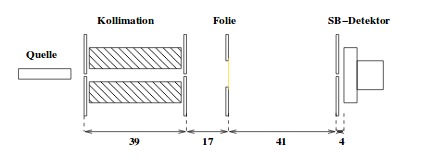
\includegraphics[width=0.7\textwidth]{aufbau}
  \caption{Der schematische Schaltplan, mit dem die Impulse
               des Zählrohres gemessen werden können. Außerdem zu sehen 
                ist ein Strommessgerät und ein Oszilloskop.
                 Die Skizze wurde aus \textcite{v703} entnommen.}
  \label{fig:aufbau}
\end{figure}
%
\subsection{Messung der Charakteristik und pro Teilchen freigesetzte Ladungsmenge}
%
Zur Messung der Charakteristik des Geiger-Müller-Zählrohres wird für
\num{14} verschiedene Spannungen zwischen Anodendraht und
Kathodenmantel, welche von \SI{320}{\volt} bis \SI{700}{\volt}
eingestellt werden, die Impulsanzahl und die Stromstärke gemessen.
Dabei werden die Impulse in einer Zeitspanne von je \SI{120}{\second}
gezählt.

Die hierbei verwendete $\beta$-Strahlenquelle wird in einem solchen
Abstand eingesetzt, dass bei einer angelegten Spannung von
\SI{320}{\volt} ca. \num{100} Impulse pro Sekunde gemessen
werden. Dadurch sollen Totzeitkorrekturen vermieden werden.  Die
Stromstärkemessung dient der Ermittlung der freigesetzen Ladungsmenge
pro registriertem Teilchen. In Formel~\eqref{eq:ladungsmenge} ist der
Zusammenhang zwischen gemessener Stromstärke $I$, Ladungsmenge $Q$ und
Teilchenzahl pro Zeit $\frac{Z}{\Delta t}$ angegeben.
\begin{equation}
I = \frac{Z}{\Delta t} Q
\label{eq:ladungsmenge}
\end{equation}
%
\subsection{Nachentladungszeitmessung}
%
Diese Messung wird mithilfe des in Abb.~\ref{fig:aufbau} gezeigten
Oszilloskops durchgeführt. Die Ablenkgeschwindigkeit des Kathodenstrahls
wird hierbei so eingestellt, dass ein Zentimeter, bzw. ein Kästchen,
einer Zeit von \SI{50}{\micro\second} entspricht. Das Oszilloskop wird
mit der Anstiegsflanke der Zählrohrimpulse getriggert.

Die Strahlungsquelle wird bei \SI{350}{\volt} in einer solchen
Entfernung zum Zählrohr angebracht, dass neben dem durch ein
registriertes Teilchen hervorgerufenen Impuls kein, oder kaum ein,
weiteres Teilchen während der Auslenkung des Kathodenstrahls über den
gesamten Oszilloskopenschirm registriert wird.

Nun wird die Spannung auf \SI{700}{\volt} erhöht, sodass es zu
Nachentladungen kommt.  Am Oszilloskop wird nun der Abstand zwischen
Primär- und Nachentladungspeak abgelesen.
%
\subsection{Totzeitmessung}
Um die Totzeit des verwendeten Zählrohres zu bestimmen werden in diesem
Versuch zwei Methoden verwendet, die nun präsentiert werden.
\subsubsection{Mit einem Oszilloskop}
%
Die Totzeitbestimmung mithilfe eines Oszilloskops verläuft beinahe
analog zur Nachentladungszeitmessung. Bei der Totzeitmessung wird
allerdings die Strahlenquelle so nahe wie möglich an das Zählrohr
angebracht, um eine hohe Strahlenintensität im Zählrohr zu erhalten.

Bei \SI{700}{\volt} Spannung am Zählrohr wird das getriggerte
Oszilloskopenbild betrachtet. An diesem wird nun abgelesen, ab welcher
Zeit nach dem Registrieren eines Teilchen das Zählrohr wieder zum
Erzeugen eines Impulses fähig ist.

Es wird hierbei auch direkt eine Messung zur Erholungszeit des
Zählrohres durchgeführt.  Dazu wird die interne Zeitablenkung auf
\SI{100}{\micro\second} erhöht, um festzstellen, ab wann wieder die
ursprüngliche Impulshöhe erreicht wird.
%
\subsubsection{Mit der Zwei-Quellen-Methode}
%
Bei der Zwei-Quellen-Methode werden drei Messungen durchgeführt.  Als
erstes wird eine Quelle 1 so nah wie möglich an das Zählrohr angebracht,
woraufhin bei einer angelegten Spannung von \SI{500}{\volt} die vom
Zählrohr in einer Zeitspanne von \SI{180}{\second} registrieren Impulse
gezählt werden.

Anschließend wird eine weiter Quelle 2 vor das Zählrohr gesetzt, sodass
die Strahlung beider Quellen registiert werden kann. Die Messung, welche
bei Quelle 1 durchgeführt wurde, wird wiederholt.  

Zum Schluss wird Quelle 1 entfernt, sodass nur noch die von Quelle 2
emittierten Teilchen vom Zählrohr registriert werden. Die Messung wird
ein weiteres mal wiederholt.  Aus den erhaltenen Impulsen und der
Messzeit lassen sich nun die registierten Impulse pro Zeit $N_1$ für
Quelle 1, $N_2$ für Quelle 2 und $N_{1+2}$ für beide Quellen zusammen
errechnen. Mit Formel~\eqref{eq:zwei_quellen} wird nun die Totzeit des
Zählrohres bestimmt.
%
\begin{equation}
\frac{N_{1+2}}{1- TN_{1+2}} = \frac{N_1}{1 - TN_1} + \frac{N_2}{1- TN_2}
\label{eq:zwei_quellen}
\end{equation}
%
Gilt $1 \gg T^2N_i^2$, so kann Formel~\eqref{eq:zwei_quellen} auch zu
Formel~\eqref{eq:zwei_quellen_naeherung} genähert werden.
%
\begin{equation}\label{eq:zwei_quellen_naeherung}
  T \approx \frac{N_1 + N_2 - N_{1+2}}{2N_1N_2}
\end{equation}

\FloatBarrier
